\documentclass{article} % This command is used to set the type of document you are working on such as an article, book, or presenation

\usepackage{geometry} % This package allows the editing of the page layout
\usepackage{amsmath}  % This package allows the use of a large range of mathematical formula, commands, and symbols
\usepackage{graphicx}  % This package allows the importing of images
\usepackage{tabularx}
\usepackage[square,numbers]{natbib}
\usepackage {hyperref}
\usepackage{fancyhdr}
\pagestyle{fancy}
\usepackage{listings}
\usepackage{appendix}
\usepackage{subcaption}
\usepackage{wrapfig}
\usepackage{fancyvrb}
\usepackage{verbatim}
\usepackage{pmboxdraw}
\usepackage[dvipsnames]{xcolor}

\usepackage{fancyvrb}

% redefine \VerbatimInput
\RecustomVerbatimCommand{\VerbatimInput}{VerbatimInput}%
{fontsize=\footnotesize,
 %
 frame=lines,  % top and bottom rule only
 framesep=10px, % separation between frame and text
 rulecolor=\color{Gray},
 %
 label=\fbox{\color{Black}modified\_architecture.txt},
 labelposition=topline,
 %
 commandchars=\|\(\), % escape character and argument delimiters for
                      % commands within the verbatim
 commentchar=*        % comment character
}

\setcitestyle{square}
\bibliographystyle{abbrvnat}

\newcommand{\maketitletwo}[2][]{
\begin{center}
        \Large{\textbf{Assignment 3 - #2}
            
            CV701 - Human and Computer Vision} % Name of course here
        \vspace{5pt}
        
        \normalsize{Khalil Alblooshi, Yevheniia Kryklyvets,
                    Sebastian Cavada, Mohamed Insaf Ismithdeen  % Group Member Names
        
        }      
        \vspace{10pt}       
\end{center}
}

\newcommand{\outlineitem}[2][]{
	#1. #2 \\ \hline 
}

% Header Logo
\setlength\headheight{39pt}
\fancyhead[L]{{\large{CV701}}}
\rhead{
\includegraphics[width=5cm]{./images/thumbnail-MBZUAI-Logo}}

\begin{document}

\maketitletwo[1]{IS2U}  % Change the group name here

\section*{Task 1 - Architectural Changes}

Neural Networks are functional units of Deep Learning, a Machine Learning technique, that are known for mimicking human brain activities in order to solve complex data-driven tasks. Important emphasis was put on the "data-driven" part of the definition since each model architecture varies depending on the given input. It was important to secure this information before applying any architectural changes, since, as was noted before, they should all be justified by the data. \\
As per the input, this assignment was released with the ImageWoof dataset, which is a subset of 10 dog breed classes from ImageNet. After analyzing provided data it was evident that the model will tend to misclassify particular classes more than the others, since differences between some breeds are so subtle, that humans were also mislabeling some inputs. Other details that were crucial to be aware of included, but were not limited to, different image sizes (resizing should be included as the pre-processing step) and the presence of images that contained multiple dogs on it (which could be easily misclassified).

\subsection*{Task 1.1 - Run base model and define optimal for it set of hyperparameters}

Together with the data each group received an initial structure for the future \textcolor{red}{?}
 Convolutional Neural Network (CNN). CNN is a kind of network architecture that is used for image recognition and tasks that include the processing of pixel data. \\
Forward pass for the given model consisted of two major blocks: feature extractor and classifier. Within the first part, there were 3 blocks, each consisting of two convolutions, with a Rectified Linear Unit (ReLU) activation function after each with one pooling layer completing the block. The classifier consisted of four linear layers with ReLU after the first three, since the last one was final, bringing us to the classification output for the ten given classes. \\
To be able to train and test the model it was important to add responsible for it code blocks: data loaders, train, evaluation, and test loops, appendix \ref{app:trainingLoop}.
For the initial run of the model, it was necessary to select hyperparameters - number of neurons, activation function, optimizer, learning rate, batch size, and epochs - that would already represent the data to reach optimal parameters faster. As per the task description, here it was important not to modify a number of neurons and activation function, since they would be changed with the architecture if required. Below you can find the table \ref{table:1} describing an initial set of hyperparameters and the results they provided:

\begin{table}[h!]
\centering
\begin{tabular}{ | c | c | c | c | }
\hline
 Optimizer & SGD  & SGD & SGD\\ 
 \hline
 Number of epochs & 50 & 50 & 50 \\  
 \hline
 Learning rate & 0.00001  & 0.0001 & 0.001 \\
 \hline
 Batch size & 64/128 & 64/128 & 64/128\\
 \hline
\end{tabular}
\caption{Initial training hyperparameters.}
\label{table:1}
\end{table}


For the first set of tests, it was decided to go with, what seemed at the moment, as close to the ground truth parameters. Stochastic gradient descent (SGD) was chosen for the optimizer since it tends to avoid local minima, computationally and memory efficient; 50 as the value for the number of epochs was chosen because it was maximum allowed value for this entry; batch size was chosen based on the general rules (power of two) and data input size; for the learning rate a grid search was performed with rather small initial values to allow the model to learn a more optimal set of weights, but with a time cost.
Those tests have proven the initial assumption wrong - the model was not learning. At this stage it was clear that the number of channels retrieved by the convolution layer was not big enough to get a minor difference between the dog breeds, thus train and validation accuracy rates were around 10\%, which with the given number of classes meant that the model was no better than random guessing. To better analyze the state of the model, a plot with training and validation accuracies was introduced, which has shown that the model was heavily overfitting on training data \ref{fig:trainBase}. After coming to this conclusion it was decided to run tests with the same set of hyperparameters, but changing the optimizer to Adam (can handle sparse gradients on noisy problems, since it utilizes momentum to accelerate the gradient descent algorithm by taking into consideration the 'exponentially weighted average' of the gradients) and AdamW (weight decay regularization added by the algorithm acts as a penalty term on the magnitude of the weights, which combining with optimal learning rate can prevent overfitting). Below are graphs \ref{fig:trainBase} that showcase the results of those tests.

\begin{figure}[h!]
    \begin{subfigure}[b]{0.43\textwidth}
         \centering
         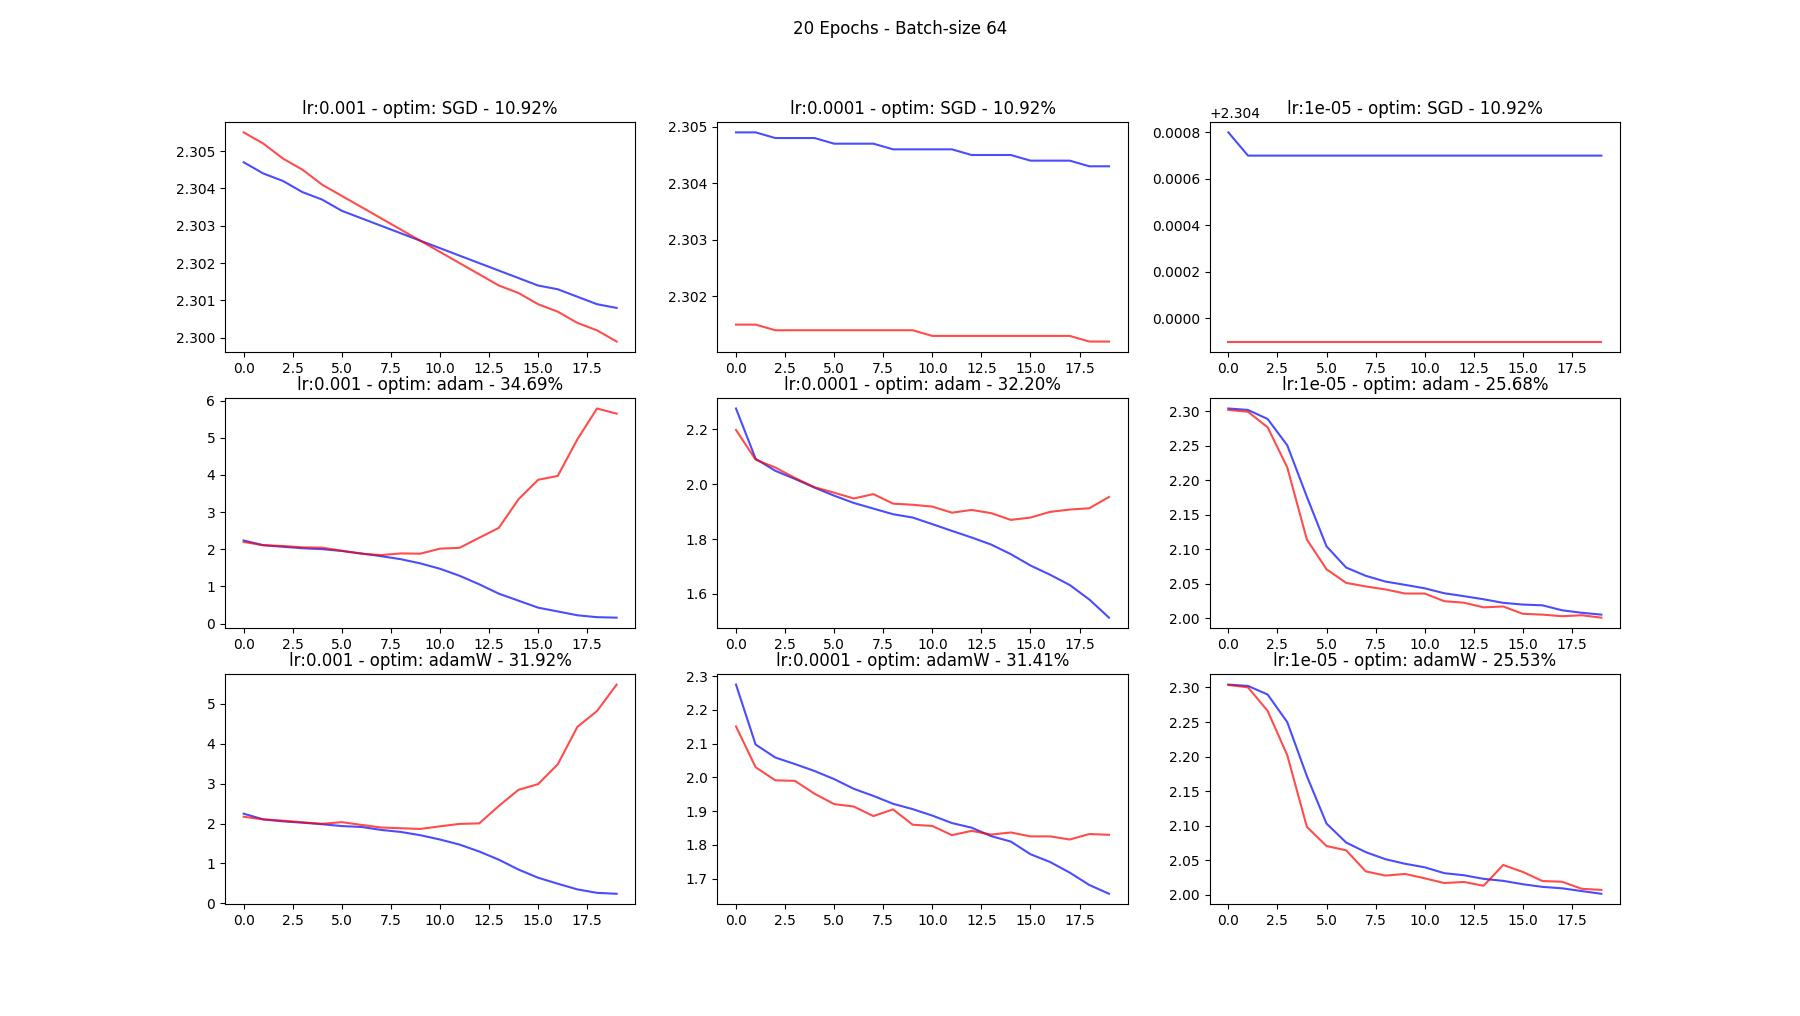
\includegraphics[scale=0.15]{./images/task_1/search_64}
         \caption{Tests performed with batch size 64}
         \label{fig:batch64}
    \end{subfigure}
    \hfill
    \begin{subfigure}[b]{0.43\textwidth}
        \centering
         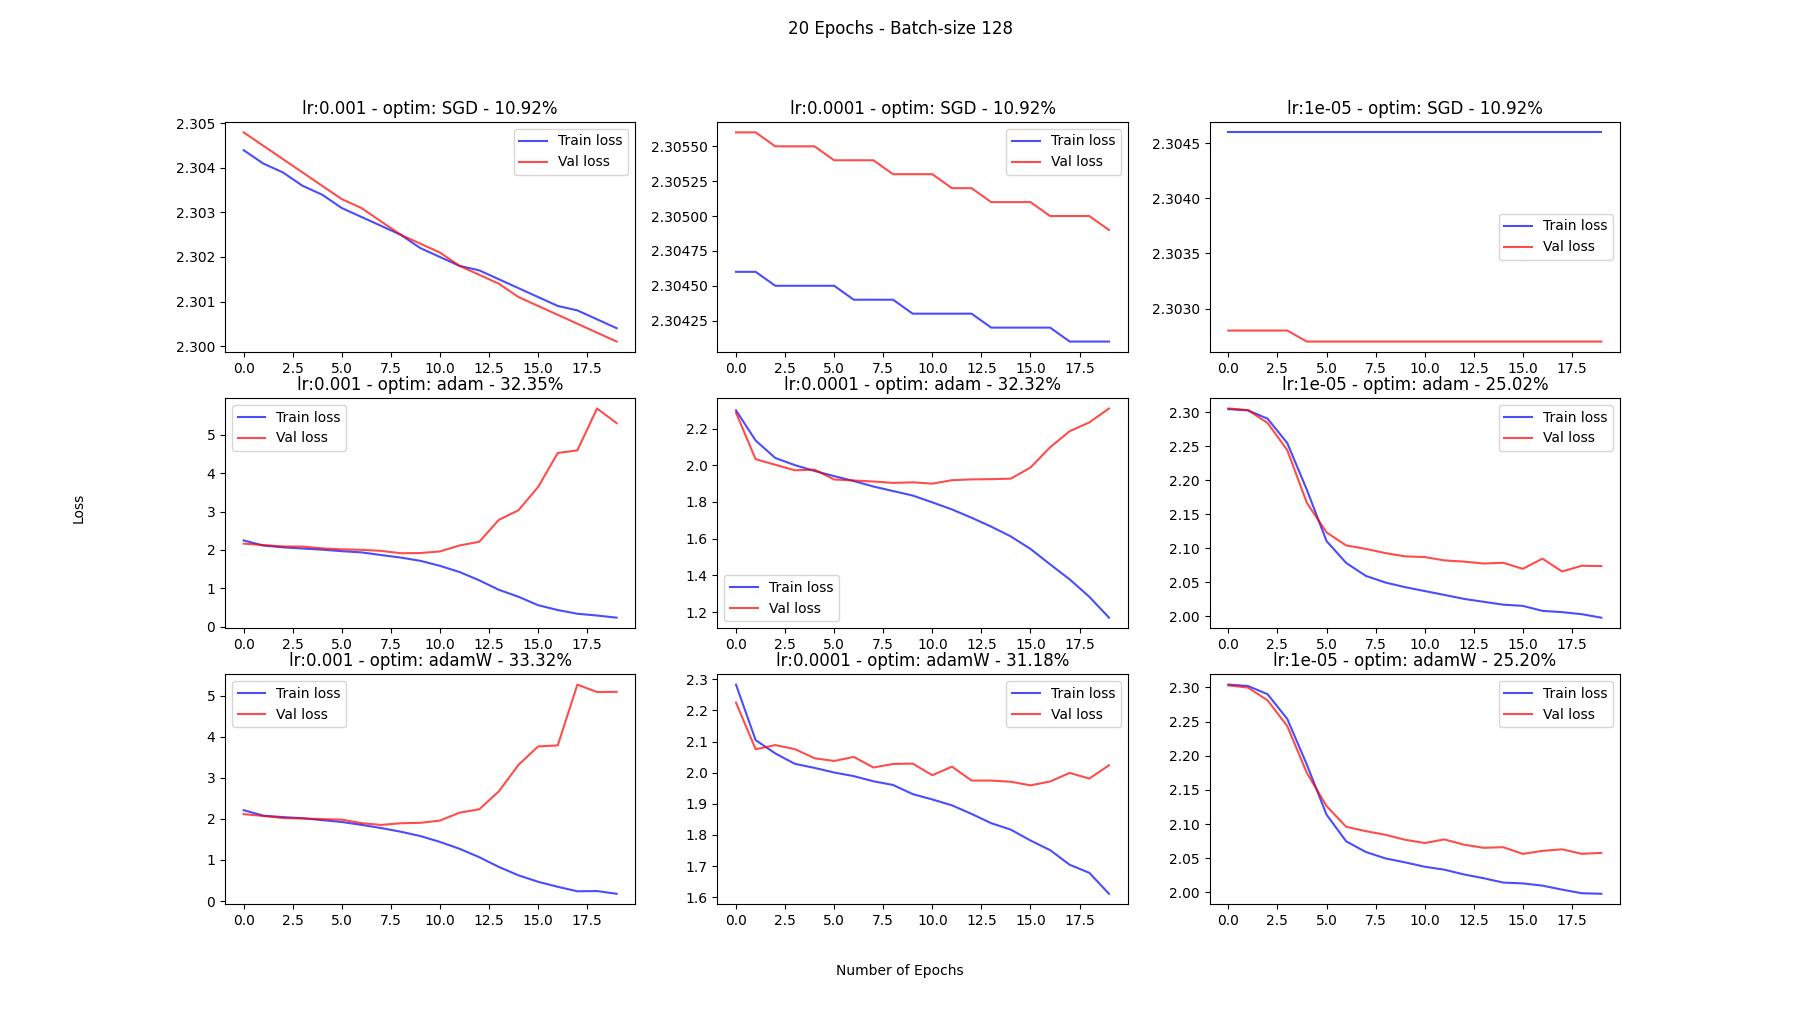
\includegraphics[scale=0.15]{./images/task_1/search_128}
         \caption{Tests performed with batch size 128}
         \label{fig:batch128}
    \end{subfigure}
    \caption{Tests performed on base model to find optimal hyperparameters}
    \label{fig:trainBase}  
\end{figure}

After the optimizer change the model was finally able to start training. After some closer examinations, it was easy to define and lock a set of the hyperparameters - table \ref{table:2} - that resulted in the best validation accuracy - 34.25\% \ref{app:bestBase}.

\clearpage

\begin{table}[h!]
\centering
\begin{tabular}{ | c | c | }
\hline
 Optimizer & Adam\\ 
 \hline
 Number of epochs & 50 \\  
 \hline
 Learning rate & 0.001 \\
 \hline
 Batch size & 64\\
 \hline
\end{tabular}
\caption{Set of optimal hyperparameters for the base model}
\vspace{-20pt}
\label{table:2}
\end{table}


\subsection*{Task 1.2 - Showcase train and test accuracy for the base model}

This subtask put the actual test set through the tuned CNN. The test set was balanced, consisting of ~415 images for each class. Below you will be able to find a chart \ref{fig:testTunedBase} displaying train and validation results for each epoch, as well as percentage showcasing accuracy on the test set. Full output can be found in appendix \ref{app:bestBase}.


\begin{figure}[h!]
    \centering     
    \includegraphics[scale=0.5]{./images/task_1/all.png} 
    \caption{Train and validation results for the tuned model showcasing accuracy on test}
    \label{fig:testTunedBase}
\end{figure}

Here we would like to note that for the entire set of experiments, it was important to use "seed". The concept of seed allows making the randomness of data more predictable. The idea behind lies in the seed being a number or a vector used to initialize a pseudorandom number generator that will affect all random numbers in the model - weights and biases, regularization in Dropout layers, and optimization techniques. This will allow for a result reproduction every time the model is run by producing the same pattern of numbers \ref{app:seed}.

\subsection*{Task 1.3 - Modify model architecture to improve performance}

After the baseline was brought to a sub-optimal state using only tuning, it was time to start architectural changes following the same goal - improve classification accuracy on the test set. From the beginning it was rather obvious that to improve classification results it was important to increase number of features to allow for a focus on actually getting down to the important feature distinction, since the original baseline stopped on 32 channels, which could be considered a lower acceptance boundary for CNNs. Another noted issue that could have contributed to the poor accuracy score was big convolution filter size for the first layer. Having this information we made an assumption that we should be able to improve model accuracy by finding an optimal trade-off between feature extractor and classifier - with a good extractor there is no need for a complicated and deep classifier. To support the theory we referred to multiple papers, some of which focused on the architecture and scaling of CNNs in general \cite{tan2019efficientnet}, while others were tackling similar classification tasks \cite{AGARWAL2020293}. After extensive review, it was decided that it should be possible to create a deeper (more layers) and wider (more neurons) model that will not break through the 3M parameter limit. \\
There are many variations of the CNN that could be implemented, thus several variations of
CNN architecture were designed and evaluated. 
Provided figure and appendices, figure \ref{fig:improvedArchitecture} and appendix \ref{app:improvedArchitecture}, showcase the best architecture of CNN, it was built following our analysis with complete layer-by-layer breakdown and the number of trainable parameters in each particular step and total, bringing us to a little over 2M parameters.

\begin{figure}[h!]
    \centering     
    \includegraphics[scale=0.45]{./images/task_1/CNN_2.png} 
    \caption{Improved architecture of the base model}
    \label{fig:improvedArchitecture}
\end{figure}


By implementing these changes we both made our model deeper and wider, which are some known approaches to improve performance of CNNs \cite{tan2019efficientnet}. It was proven that the balance of these scaling values are dependent on each other and the values would change under different constraints. To finalize the decision about the model it was important to run again train-validation-test circle to be sure about the performance. At this stage, test accuracy went up to 41\%.

\subsection*{Task 1.4 - Add Dropout and Batch Normalization layers}

In order to finalize the structure of the ConvNet it was important to add Dropout and Batch Normalization layers to solve some major issues in the model. All deep neural networks tend to have an internal covariate shift problem, which is defined as a change in the distribution of each layer’s inputs, due to the change in parameters after each layer. To manage this problem batch normalization was introduced in the model to basically normalize all inputs using zero mean and unit variance. It results in multiple benefits for the deeper networks, allowing for a higher learning rate and faster training time, being less careful with the weight initialization, which becomes a more complicated task with the network depth and provides a bit of regularization. This results in improved overall performance for the model, since the model converges faster, taking bigger gradient steps. It is important to state that batch normalization layers have to be implemented before activation functions, which ensures that the normalization is appropriately handled by any optimization method that is being used to train the network \cite{ioffe2015batch}. This increased accuracy in 1.5 times, bringing performance on the test set to \emph{Test loss: 1.4267 Accuracy: 61.26\%}. \\
Another issue that this model presented was complex co-adaptations of the feature detectors since some differences between the breeds were so subtle. Dropout addresses this issue by randomly omitting some percentage of feature detectors on each training set, thus enabling neurons to learn to detect a feature that is actually helpful for producing the correct answer. To improve performance different approaches were tried. Taking inspiration from the paper \cite{hinton2012improving}, we started with adding dropout layers with 50\% probability value after all convolutional layers. It was expected that the model would have worse accuracy since we are now skipping many features. \emph{Accuracy: 21.61\%} has proven original assumptions. A simple reduction of the probability value to 20\% has shown not to be a viable option as well, still, there seemed to be not enough distinctive features to learn. This has shown that dropout should be added only for the last convolution layers, where number of total features was significant and detailed enough to omit \cite{inproceedings}, and in front of each linear projection \cite{JMLRv15srivastava14a}. 
These changes have finalized the model architecture with the following \emph{Test loss: 2.0502 Accuracy: 64.90\%}. The model we were now observing, appendix \ref{app:finalArchitecture}, required additional parameter tuning, not only because introduced dropout slowed convergence rate, but also due to the fact that was stated earlier - a set of hyperparameters is unique to the task and the model. After all the introduced changes there was almost no trace of the original model. This brings us to the following task.

\section*{Task 2 - Hyperparameter Changes}

\subsection*{Task 2.1 - Different optimizers experimentation}
In addition to SGD, adam, and adamW, trials of several optimizers were carried into the model, where results articulated high and low performances on a fixed learning rate of 0.0.1 and an epoch of 20. 


\begin{table}[h!]
\centering
\begin{tabular}{ | c | c | c | c | c | }
\hline
 Optimizer: & adadelta & nadam & adagrad & asgd\\
 \hline
 Accuracy: & 0.1 \% & 0.05 \% & 0.1 \% & 0.05 \%\\
 \hline
 Loss: & 57.75 & 60.17 & 63.30 & 63.30\\
 \hline
\end{tabular}
\caption{Various optimizers performance}
\label{table:91}
\end{table}



For instance, the ...(SGD, Adam, ... ) increased the (accuracy/reduced loss/...), yet the time has increased/decreased slightly as this optimizer ...(explain it). 
On the other hand, (SGD, Adam, ...) did not have a huge influence on the model accuracy in comparison to (SGD/Adam/...). In addition, ...(SGD, Adam, AdamW) is known for its ...., here it is evident that it entailed the model to behave the same as when applying (SGD, Adam, AdamW), yet on the condition of high learning rate it showed better/less performance.



\subsection*{Task 2.2 - Learning rate and learning rate scheduler experiments}


We experimented with 3 learning rates.
For all the experiments in Table \ref{table:3}; Epochs=50, Optimizer=Adam and batch\_size=64 was used.

\begin{table}[h!]
\centering
\begin{tabular}{ | c | c | c | c |}
\hline
 LR  & 0.1 & 0.01 & 0.001\\
 \hline
 Test accuracy & 10.41\% & 54.98\% & 61.59\%\\
 \hline
\end{tabular}
\caption{Variation of Test Accuracy with Learning Rate}
\label{table:3}
\end{table}


\begin{figure}[h!]
	\centering
	\begin{subfigure}{0.32\linewidth}
		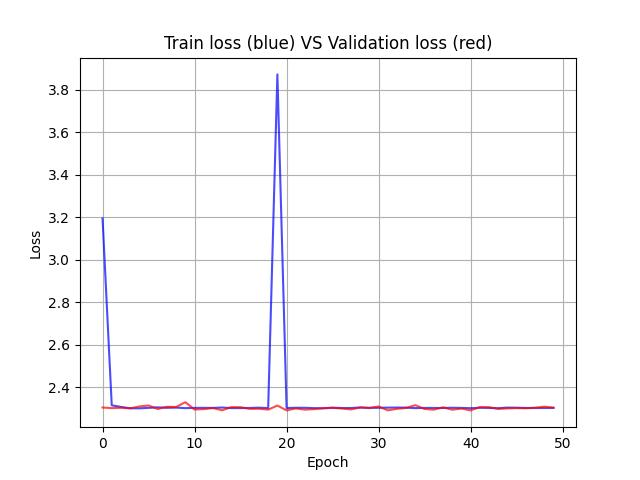
\includegraphics[width=\linewidth]{Assignment_Submission_Template/images/task_2/2.2/results_e50_l0.1_adam_model06_ReLUtrainloss.jpg}
		\caption{LR = 0.1}
		\label{fig:LR0.1}
	\end{subfigure}	
        \begin{subfigure}{0.32\linewidth}
		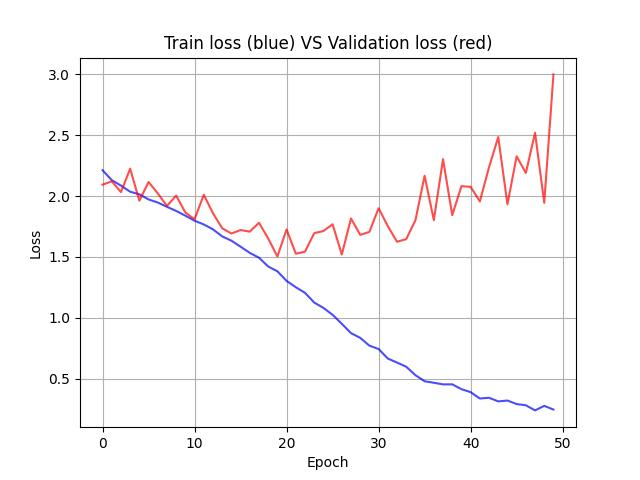
\includegraphics[width=\linewidth]{Assignment_Submission_Template/images/task_2/2.2/results_e50_l0.01_adam_model06_ReLUtrainloss.jpg}
		\caption{LR = 0.01}
		\label{fig:LR0.01}
	\end{subfigure}	
	\begin{subfigure}{0.32\linewidth}
	        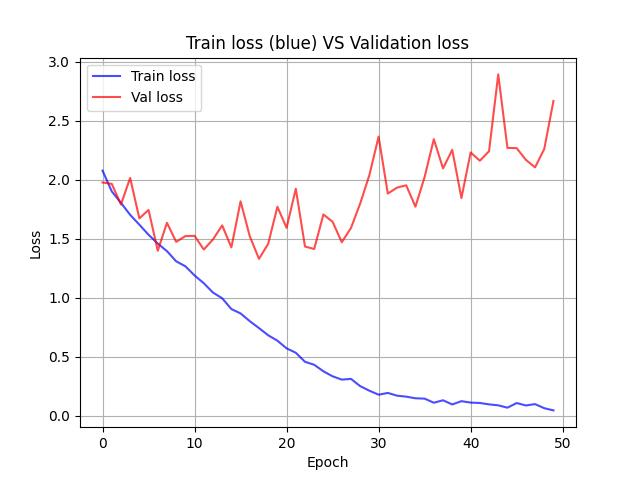
\includegraphics[width=\linewidth]{Assignment_Submission_Template/images/task_2/2.2/results_e50_l0.001_adam_model06_ReLUtrainloss.jpg}
	        \caption{LR = 0.001}
	        \label{fig:LR0.001}
         \end{subfigure}
	\caption{Different LR}
	\label{fig:subfigures}
\end{figure}



We experimented with two types of Learning rate schedulers in Pytorch; StepLR and ReduceLROnPlateau as follows.

\textit{scheduler = torch.optim.lr\_scheduler.StepLR(optimizer,step\_size=10, gamma=0.1)} 

\textit{scheduler = torch.optim.lr\_scheduler.ReduceLROnPlateau(optimizer, mode='min', factor=0.1)} 

Validation Loss was used as the metric for ReduceLROnPlateau.

For all the experiments in Table \ref{table:4}; Epochs=50, Optimizer=Adam, batch\_size=64 and Initial Learning Rate=0.01 was used.

\begin{table}[h!]
\centering
\begin{tabular}{ | c | c | c | c | c | }
\hline
 LR Scheduler & (a)StepLR & (b)StepLR & (c)ReduceLROnPlateau & (d)ReduceLROnPlateau\\
 \hline
 Gamma/Factor & 0.1 & 0.05 & 0.1 & 0.05\\
 \hline
 Step size & 20 & 10 & N/A & N/A\\
 \hline
 Test accuracy & 57.75\% & 60.17\% & 63.30\% & 63.30\%\\
 \hline
\end{tabular}
\caption{Variation of Test Accuracy with Learning Rate Scheduler}
\label{table:4}
\end{table}

\begin{figure}[h!]
	\centering
	\begin{subfigure}{0.25\linewidth}
		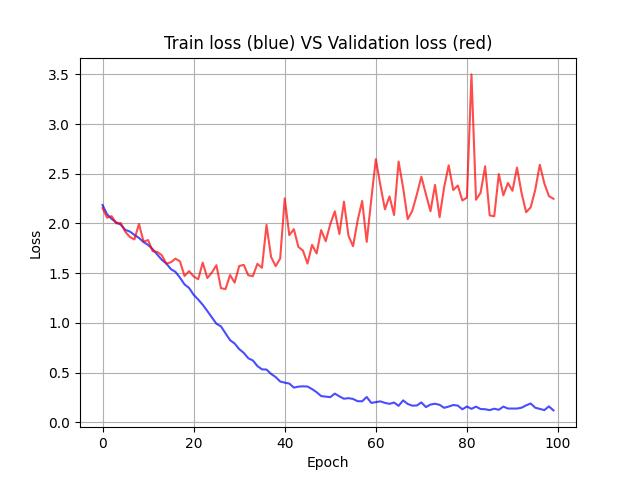
\includegraphics[width=\linewidth]{Assignment_Submission_Template/images/task_2/2.2/results_e100_l0.01_adam_model06_ReLU_StepLR(step_size=10,gamma=0.05,epochs=50)trainloss.jpg}
	    \caption{}
		\label{fig:StepLR(step_size=10,gamma=0.05)}
	\end{subfigure}	
        \begin{subfigure}{0.25\linewidth}
		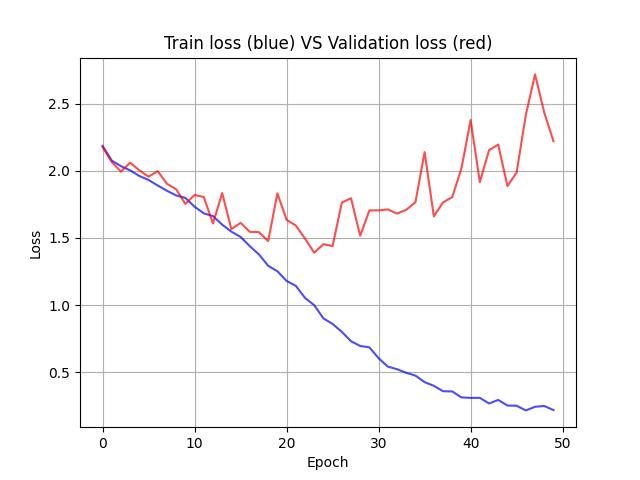
\includegraphics[width=\linewidth]{Assignment_Submission_Template/images/task_2/2.2/results_e50_l0.01_adam_model06_ReLU_StepLR(step_size=20,gamma=0.1,epochs=50)trainloss.jpg}
		\caption{}
		\label{fig:StepLR(step_size=20,gamma=0.1)}
	\end{subfigure}	
	\begin{subfigure}{0.25\linewidth}
	        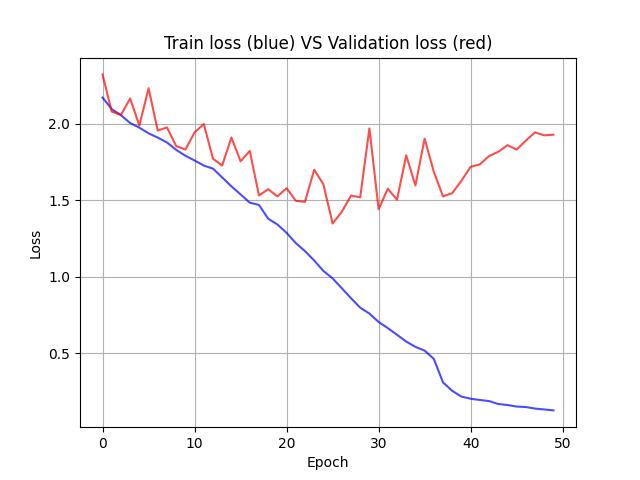
\includegraphics[width=\linewidth]{Assignment_Submission_Template/images/task_2/2.2/results_e50_l0.01_adam_model06_ReLU_ReduceLROnPlateau(factor=0.05,epochs=50)trainloss.jpg}
	        \caption{}
	        \label{fig:ReduceLROnPlateau(factor=0.05)}
         \end{subfigure}
         \begin{subfigure}{0.25\linewidth}
	        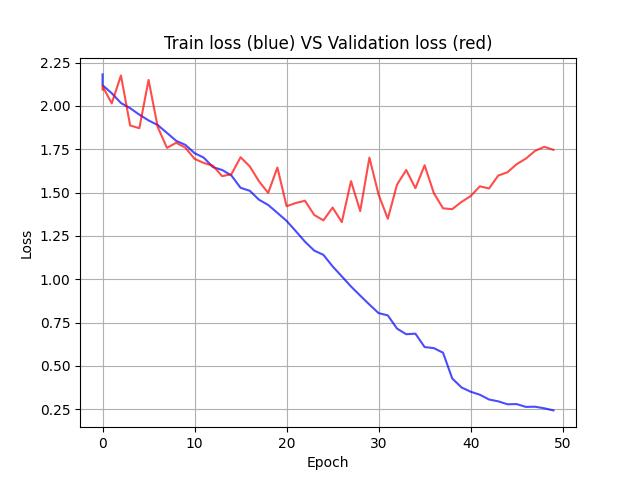
\includegraphics[width=\linewidth]{Assignment_Submission_Template/images/task_2/2.2/results_e50_l0.01_adam_model06_ReLU_ReduceLROnPlateau(factor=0.1,epochs=50)trainloss.jpg}
	        \caption{}
	        \label{fig:ReduceLROnPlateau(factor=0.1)}
         \end{subfigure}
	\caption{Different LR Schedulers}
	\label{fig:subfigures}
\end{figure}


\subsection*{Task 2.3 - Analysis on different epochs and batch sizes}

This part of the assignment was focused on two important hyperparameters that are crucial for performance. Number of epochs is directly related to over- or underfitting - when the value is too small model is unable to capture underlying patterns in the data, while too many of them result in the model being too specific to the training data, which reflects poor generalization. Batch size is important because it affects both the training time and the generalization of the model. Smaller batch size increases training time, but allows for learning from each individual example, while increasing this value will shorten the training time, but might lead to missing important data nuances. With this information in mind, we were able to form our original assumptions: 
\begin{itemize}
  \item Since 20 epochs that were used previously did not provide enough convergence rate, we should go bigger to allow the model enough time to learn.
  \item For the learning rate tests 50 epochs provided the best outcome, so this value has to be included in tests (also because it is the highest allowed value and we cannot just  omit it from the testing)
  \item Since we are in the lab environment, for the batch size we can allow for the smaller numbers, for instance, starting with 32, to let the model train more thoroughly.
  \item Batch size 64 has shown to be optimal in all previous tests, so it also was included in this round of fine-tuning.
  \item It was also very interesting to test out the theory that it is not necessary to select batch size that is in the power of 2, since the fact that it improves efficiency from the computational perspective could be outdated \cite{Raschka_2022}. That's why we decided to pick 45 as the third value for batch size.
\end{itemize}
The original hypothesis was next: best accuracy will be provided by the model that will run for 50 epochs (more time to learn) and will be training on a batch size 32 (or 45, since it's a ``dark horse" situation) since it allows for learning before seeing all data.

\subsection*{Task 2.4 - Effect of data augmentation}

For this task, the data augmentation technique that was used is: "CutMIX" \cite{yun2019cutmix}. It is a very popular and powerful technique that randomly cuts part of an image and replaces it with another image in the same batch. It is an improved version of the Cutout technique because it allows for less information loss, and improves the robustness of the algorithm. The implementation of PyTorch was used \cite{cutmixpytorch} and our code had to be slightly modified to enable the new data augmentation. The technique is made up of two sub-techniques each one that applies a slightly different data augmentation. On the right it can be specifically seen that the image is cut and replaced with a different part of another image; on the left instead, an image is overlaid on top of the original with different opacity levels. The ground truth is therefore not just a single label anymore, but rather a probability of finding some class in the augmented image. Usually, only two classes are present in each image.
As stated at the beginning, this model is advanced and its strength relies on the ability to "enhance localization ability by requiring the model to identify the object from a partial view" \cite{yun2019cutmix}. The choice to apply this technique was twofold Firstly being advanced it enabled us to dig deeper into the different augmentation techniques. Furthermore, it gave us some insights into how some training is made and tried to give us the chance to understand the important point that needs to be addressed in data augmentation.

In the last step, the accuracy reached 67\%.

\begin{table}[h!]
\centering
\begin{tabular}{ | c | c | c | }
\hline
 added & Accuracy & Improvement \\ 
 \hline
 Baseline & 10\% & - \\   
 Changing optimizer & 27\% & 17\% \\ 
 Changing architecture & 47.54\% & 20\%\\
 Batch normalization &  61.26\% & 14\% \\
 Dropout & 65.18\% & 4\% \\
 Augmentation & 67.60\% & 2.5\%\\
\hline
\end{tabular}
\caption{Improvements to the base model and relative accuracy}
\vspace{-20pt}
\label{table:2}
\end{table}

\begin{figure}[h!]
	\centering
	\begin{subfigure}{0.5\linewidth}
		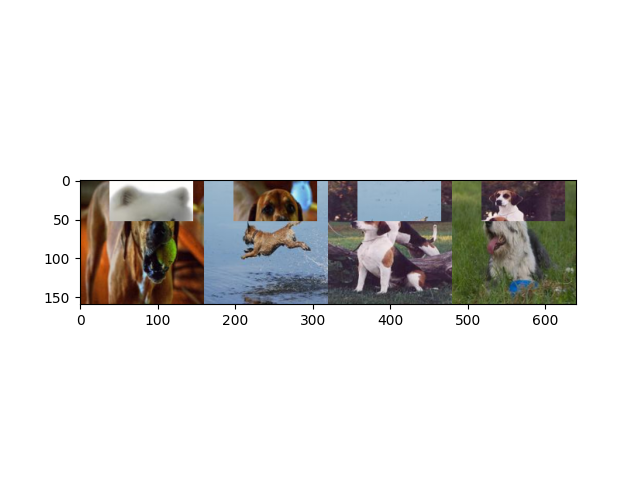
\includegraphics[width=\linewidth]{Assignment_Submission_Template/images/task_2/augment.png}
		\caption{Cut technique}
		\label{fig:subfigA}
	\end{subfigure}	
	\begin{subfigure}{0.49\linewidth}
	        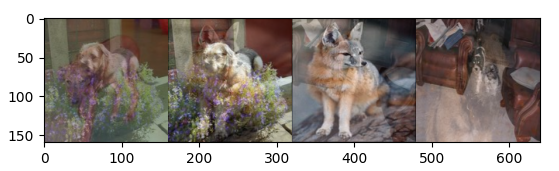
\includegraphics[width=\linewidth]{Assignment_Submission_Template/images/task_2/augment_2.png}
	        \caption{Mix Technique}
	        \label{fig:subfigC}
         \end{subfigure}
	\caption{Different approaches in the CutMIX technique.}
	\label{fig:subfigures}
\end{figure}

\clearpage
\bibliography{references}
\clearpage

\appendix

\section*{Appendices}

\section{Output for the best base model performance}
\label{app:bestBase}
\begin{lstlisting}
0 train loss: 2.2358 accuracy: 14.1943
 val loss: 2.1957 accuracy: 16.5188 best_accuracy: 0.0000
1 train loss: 2.1090 accuracy: 20.0788
 val loss: 2.1098 accuracy: 20.1774 best_accuracy: 16.5188
2 train loss: 2.0670 accuracy: 22.5040
 val loss: 2.0877 accuracy: 21.2860 best_accuracy: 20.1774
3 train loss: 2.0273 accuracy: 24.3506
 val loss: 2.0514 accuracy: 23.6142 best_accuracy: 21.2860
4 train loss: 2.0030 accuracy: 25.4709
 val loss: 2.0437 accuracy: 22.0621 best_accuracy: 23.6142
5 train loss: 1.9539 accuracy: 27.5637
 val loss: 1.9592 accuracy: 26.9401 best_accuracy: 23.6142
6 train loss: 1.8874 accuracy: 29.5827
 val loss: 1.8781 accuracy: 28.6031 best_accuracy: 26.9401
7 train loss: 1.8141 accuracy: 33.2390
 val loss: 1.8432 accuracy: 31.9290 best_accuracy: 28.6031
8 train loss: 1.7329 accuracy: 37.0183
 val loss: 1.8883 accuracy: 29.7118 best_accuracy: 31.9290
9 train loss: 1.6198 accuracy: 41.2902
 val loss: 1.8809 accuracy: 31.7073 best_accuracy: 31.9290
10 train loss: 1.4747 accuracy: 46.2883
 val loss: 2.0167 accuracy: 32.1508 best_accuracy: 31.9290
11 train loss: 1.2858 accuracy: 53.9333
 val loss: 2.0389 accuracy: 34.2572 best_accuracy: 32.1508
12 train loss: 1.0564 accuracy: 62.1199
 val loss: 2.3095 accuracy: 32.8160 best_accuracy: 34.2572
13 train loss: 0.8034 accuracy: 71.0944
 val loss: 2.5769 accuracy: 30.2661 best_accuracy: 34.2572
14 train loss: 0.6157 accuracy: 78.1854
 val loss: 3.3452 accuracy: 30.8204 best_accuracy: 34.2572
15 train loss: 0.4272 accuracy: 85.4364
 val loss: 3.8708 accuracy: 31.1530 best_accuracy: 34.2572
16 train loss: 0.3253 accuracy: 89.1173
 val loss: 3.9750 accuracy: 31.4856 best_accuracy: 34.2572
17 train loss: 0.2219 accuracy: 93.1183
 val loss: 4.9603 accuracy: 30.1552 best_accuracy: 34.2572
18 train loss: 0.1707 accuracy: 94.6818
 val loss: 5.7911 accuracy: 27.0510 best_accuracy: 34.2572
19 train loss: 0.1576 accuracy: 95.2850
 val loss: 5.6521 accuracy: 30.3769 best_accuracy: 34.2572
Test loss: 2.0686 Accuracy: 34.69%
\end{lstlisting}

\section{Code for the seed implementation}
\label{app:seed}
\begin{lstlisting}
def START_seed():
    seed = 9
    torch.manual_seed(seed)
    torch.cuda.manual_seed(seed)
    torch.cuda.manual_seed_all(seed)
    np.random.seed(seed)
    random.seed(seed)
    torch.backends.cudnn.benchmark = False
    torch.backends.cudnn.deterministic = True

\end{lstlisting}    

\section{Improved Neural Architecture}
\label{app:improvedArchitecture}
\begin{lstlisting}
class CNN(nn.Module):
    def __init__(self, num_classes=10, activation=nn.SiLU):
        super().__init__()

        self.feature_extractor = nn.Sequential(
            nn.Conv2d(3, 32, 3, 1),
            nn.ReLU(),  
            nn.MaxPool2d(2),
            #####
            nn.Conv2d(32, 64, 3, 1),
            nn.ReLU(),
            nn.Conv2d(64, 64, 3, 1),
            nn.ReLU(),
            nn.MaxPool2d(2),
            #####
            nn.Conv2d(64, 128, 3, 1),
            nn.ReLU(),
            nn.Conv2d(128, 128, 3, 1),
            nn.ReLU(),
            nn.MaxPool2d(2),
            #####
            nn.Conv2d(128, 256, 3, 1),
            nn.ReLU(),
            nn.Conv2d(256, 256, 3, 1),
            nn.ReLU(),
            nn.MaxPool2d(2),
            #####
            nn.Conv2d(256, 384, 3, 1),
            nn.ReLU(),
            nn.AdaptiveAvgPool2d(
                output_size=1,
            ),
            nn.Flatten()
        )
        self.classifier = nn.Sequential(
            nn.Linear(384, 192),            
            nn.ReLU(),
            nn.Linear(192, 64),            
            nn.ReLU(),
            nn.Linear(64, num_classes),
        )    

\end{lstlisting}

\VerbatimInput{modified_architecture.txt}

\section{Final Neural Architecture}
\label{app:finalArchitecture}
\begin{lstlisting}
class CNN(nn.Module):
    def __init__(self, num_classes=10, activation=nn.SiLU):
        super().__init__()
        
        self.feature_extractor = nn.Sequential(
            nn.Conv2d(3, 32, 3, 1),
            nn.ReLU(),          
            nn.MaxPool2d(2),
            #####
            nn.Conv2d(32, 64, 3, 1),
            nn.BatchNorm2d(64),
            nn.ReLU(),           
            nn.Conv2d(64, 64, 3, 1),
            nn.BatchNorm2d(64),
            nn.ReLU(),          
            nn.MaxPool2d(2),            
            #####
            nn.Conv2d(64, 128, 3, 1),
            nn.BatchNorm2d(128),
            nn.ReLU(),           
            nn.Conv2d(128, 128, 3, 1),
            nn.BatchNorm2d(128),
            nn.ReLU(),          
            nn.MaxPool2d(2),
            ####
            nn.Conv2d(128, 256, 3, 1),
            nn.BatchNorm2d(256),
            nn.ReLU(),           
            nn.Conv2d(256, 256, 3, 1),
            nn.BatchNorm2d(256),
            nn.ReLU(),           
            nn.MaxPool2d(2),
            ####
            nn.Conv2d(256, 384, 3, 1),
            nn.BatchNorm2d(384),
            nn.ReLU(),
            nn.Dropout(0.2),
            nn.AdaptiveAvgPool2d(
                output_size=1,
            ),
            nn.Flatten()
        )
        self.classifier = nn.Sequential(
            nn.Linear(384, 192),            
            nn.ReLU(),
            nn.Dropout(0.2),
            nn.Linear(192, 64),            
            nn.ReLU(),
            nn.Dropout(0.2),
            nn.Linear(64, num_classes),
        )
\end{lstlisting}

\section{Training loop code}
\label{app:trainingLoop}
\begin{lstlisting}

## Creating training loop
def train(model, epoch):
    model.train()
    train_loss = 0
    total = 0
    correct=0
    with tqdm(train_loader, unit="batch") as tepoch:
        for batch_idx, (data, target) in enumerate(tepoch):
            # send to device
            data, target = data.to(device), target.to(device)
    
            # clear the gradients of all optimized variables
            optimizer.zero_grad()
            # forward pass: compute predicted outputs by passing inputs to the model
            output = model(data)
            # calculate the loss
            loss = criterion(output, target)
            # backward pass: compute gradient of the loss with respect to model parameters
            loss.backward()
            # perform a single optimization step (parameter update)
            optimizer.step()
            # update running training loss
            train_loss += loss.item()
            _, predicted = output.max(1)
            total += target.size(0)
            correct += predicted.eq(target).sum().item()
            tepoch.set_postfix(loss=train_loss/(batch_idx+1), lr=optimizer.param_groups[0]['lr'])
        log = 'Epoch: {} - train loss: {:.4f} accuracy: {:.4f}\n'.format(epoch, train_loss/(batch_idx+1), 100.*correct/total)
        print(log)
        with open(path + "/log.txt", 'a') as file:
                file.write(log)


def validate(model):
    global best_accuracy
    model.eval()

    best_loss = 0
    test_loss = 0
    correct = 0
    total = 0

    with tqdm(val_loader, unit="batch") as tepoch:
        for batch_idx, (data, target) in enumerate(tepoch):
            data, target = data.to(device), target.to(device)
    
            output = model(data)
            loss = nn.CrossEntropyLoss()(output, target)
            test_loss += loss.item()
            _, predicted = output.max(1)
            total += target.size(0)
            correct += predicted.eq(target).sum().item()
        if loss > best_loss:
            print("Saving the best model...")
            best_loss = loss
            torch.save(model.state_dict(), path + '/best_model.pth')
        log = ' val loss: {:.4f} accuracy: {:.4f} best_loss: {:.4f}\n'.format(test_loss/(batch_idx+1), 100.*correct/total, best_loss)
        print(log)
        with open(path + "/log.txt", 'a') as file:
            file.write(log)        

def test_best_model(model, test_loader, criterion, best_model_path):
    # Load the best model
    model.load_state_dict(torch.load(best_model_path))
    model.eval()

    test_loss = 0
    correct = 0
    total = 0

    with tqdm(test_loader, unit="batch") as tepoch:
        for batch_idx, (data, target) in enumerate(tepoch):
            data, target = data.to(device), target.to(device)

            output = model(data)
            loss = criterion(output, target)
            test_loss += loss.item()

            _, predicted = output.max(1)
            total += target.size(0)
            correct += predicted.eq(target).sum().item()

        accuracy = 100. * correct / total        
        log = 'Test loss: {:.4f} Accuracy: {:.2f}%'.format(test_loss/(batch_idx+1), accuracy)
        print(log)
        with open(path + "/log.txt", 'a') as file:
            file.write(log)
\end{lstlisting}

\end{document}